\onehalfspacing
\section{Anforderungen}
	\subsection{Anforderungsdefinition}
Zu Beginn des Projekts werden die konkreten Anforderungen an die Suite mit dem Auftraggeber abgestimmt und in Form einer Tabelle Festgehalten. Dieses Vorgehen erleichtert die Endabnahme des Projekts, da die Anforderungen klar definiert und beiden Parteien bekannt sind. Auf die Erstellung eines gesamten \ac{SRS} wird im Rahmen dieses Projekt aus Zeitgründen bewusst verzichtet. Bei den Anforderungen wird zwischen funktionalen und nicht-funktionalen unterschieden. Funktionale Anforderungen sind all jene, welche eine konkrete Funktion der Software definieren. Nicht Funktionale Anforderungen sind Anforderungen wie z.B. Zuverlässigkeit und Zeitverhalten. Die Anforderungen sind in den Tabellen \dq \nameref{tab:Anforderungstabelle}\dq und \dq \nameref{tab:Anforderungstabelle2}\dq dargestellt.
\newpage
\begin{table}[h]
\begin{center}
\begin{tabularx}{\textwidth}{|c|X|X|c|}
\hline
Nr. & Bezeichnung & Beschreibung & Zuordnung \\
\hline
F01 & Error Codes & Eignung zur Stimulation der verschiedenen Fehlerfälle und  dadurch Produktion der entsprechenden Fehlermeldungen (01h-23h) & Funktional \\
\hline
F02 & Identifikation des DUT & Überprüfung der Firmware Version, des elektronischen Typenschilds auf Korrektheit & Funktional \\
\hline
F03 & Diagnose Funktionalität & Überprüfung der vorhandenen Diagnose Funktionalität (z.B. Spannungs Monitoring) & Funktional \\
\hline
F04 & Core Funktionalität & Prüfung der externen Temperatur Schnittstelle, sowie der Single und multiturn Positionsbestimmung & Funktional \\
\hline
F05 & Schnittstellen Config & Auslesen und überprüfen der Schnittstellen Parametrisierung und Funktionalität & Funktional \\
\hline
F06 & Hiperface Befehle & Überprüfung der Funktion der verschiedenen Hiperface Befehle sowie der entsprechnden Antwort & Funktional \\
\hline
F07 & Integration in Automated Testing & Die Suite muss in das Projekt "Automated Testing" Integrierbar sein (Implementierung in ITE, Aufbau nach Vorgaben des Projekts) & Funktional \\
\hline
\end{tabularx}
\end{center}
\caption{Anforderungen funktional \label{tab:Anforderungstabelle}}
\end{table}

\begin{table}[h]

\begin{center}

\begin{tabularx}{\textwidth}{|c|X|X|c|}

\hline
Nr. & Bezeichnung & Beschreibung & Zuordnung \\
\hline
NF01 & Externes Equipment & Möglichkeit zur Integration des am Teststand vorhandenen externe Equipment & Nicht Funktional \\
\hline
NF02 & Universell einsetzbar & Der Aufbau der Suite soll so gestaltet sein, das diese auch zukünftig für die Portierung anderer (ähnlicher) Produkte genutzt werden kann & Nicht Funktional \\
\hline
NF03 & Coding Guidelines & Der Aufbau der Suite soll so gestaltet sein, das diese auch zukünftig für die Portierung anderer (ähnlicher) Produkte genutzt werden kann & Nicht Funktional \\
\hline


\end{tabularx}
\caption{Anforderungen nicht-funktional \label{tab:Anforderungstabelle2}}
\end{center}
\end{table}
\cleardoublepage

\subsection{Analyse bisheriger Testfälle}
Zu Ermittlung der Testfälle welche durch die Suite abgedeckt werden sollen werden die bisherigen Testpläne analysiert. Schwierigkeit hierbei ist, dass der Geber vor ca. 20 Jahren entwickelt wurde. Zum Entwicklungszeitpunkt fand keine, den heutigen Standards entsprechende Dokumentation der Testfälle (Testplan) statt, weiterhin ist zum Projektstart noch kein Testplan für Portierung des Controllers vorhanden. Aus diesem Grund wird für die Analyse der Testfälle auf den Testplan eines ähnlichen Produktes (SEY) welches ebenfalls über eine Hiperface Schnittstelle verfügt zurück gegriffen.\newline
	Die im Testplan festgelegten Tests werden in eine Excel Tabelle übertragen, die Testfälle sind im Testplan in verschiedene Kategorien unterteilt (z.B. General Requirements, HW Architecture, functional Requirements). Da der SEY über zwei Mikrocontroller verfügt (Master und Slave) der SK jedoch nicht werden daraufhin die Testfälle des Slave Microcontrollers aus dem Testplan gestrichen. In einem Zweite Schritt wird die Beschreibung jedes Testfalls Analysiert und geprüft ob dieser Testfall automatisierbar ist. Ein Beispiel für einen nicht automatisierbaren Testfall ist z.B. beim Eingriff mittels Debugger während des Tests gegeben. Die verbleibenden Tests werden mit dem Zuständigen SW-Entwickler besprochen und ggf. angepasst um im folgenden als Grundlage für die Kozeptionierung dienen zu können. Die Entwicklung eines kompletten Testplans für die Portierung wird hierbei nicht forciert, da hierzu der Zeitliche Rahmen nicht gegeben ist. Die 
Analyse der Testfälle zeigt, das sich die Suite besonders für das Testen der Hiperface Schnittstelle eignet. Hier können die verschiedenen Befehle der Schnittstelle gut abgebildet werden. Die Ergebnisse der Analyse sind in \dq \nameref{fig:Analyse.jpg}\dq   Beispielhaft dargestellt und befinden sich im Anhang. Die Farbgebung der Tabelle entspricht den Testfall Clustern.
\begin{figure}[h]
	\centering
  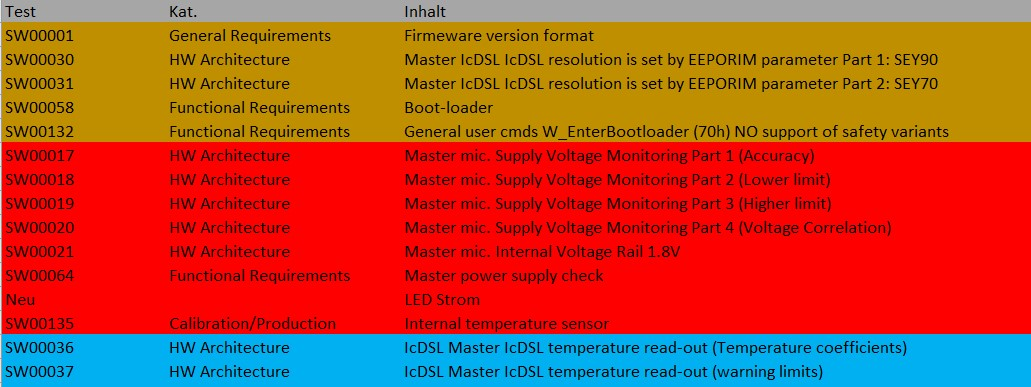
\includegraphics[width=1.25\textwidth, angle=90]{img/Tests_Cluster.jpg} 
   \caption{Tabelle mit Analysierten Testfällen}
  \label{fig:Analyse.jpg}
\end{figure}

